\chapter{Technische Details zu den Rekonstruktionen}
\label{app:param}
Die genauen für die Rekonstruktionen in \fref{chap:rekonstruktion} genutzten Abfolgen sowie die verwendeten Parameter werden die im Folgenden detailliert.

Bei den zweidimensionalen Rekonstruktionen wird zur Erzeugung des initialen Supports und der Startwerte für die IPR mit Shrinkwrap die Funktion \texttt{generic\_support} genutzt, deren Ablaufschema in \fref{fig:flow_genericsupport} dargestellt ist. Die eigentliche Rekonstruktion läuft nach dem in \fref{fig:flow_sw} dargestellten Schema ab.
Für die Erzeugung des Support und der Startwerte mittels Holographie wird die Funktion \texttt{holo\_support} genutzt, deren Ablaufschema in \fref{fig:flow_holosupport} dargestellt ist, die anschließende Rekonstruktion läuft nach dem in \fref{fig:flow_holo} dargestellten Schema ab, das bis auf die erste Phase identisch zu zum Ablauf bei Nutzung von Shrinkwrap ist.
Die jeweils genutzten Parameter sind in \fref{tab:param} aufgelistet.
Die in der Wiener-Entfaltung genutzte Kreuzkorrelation wird ebenfalls mittels \texttt{holo\_support} identifiziert. Hierbei wird jedoch der Parameter \textit{radDilate} aus \SI{50}{Pixel} erhöht, da die Entfaltung gänzlich unempfindlich gegenüber einer zu groß gewählten, jedoch äußerst empfindlich gegenüber abgeschnittenen Kreuzkorrelation reagiert. Die verwendeten Parameter $N$ der Wiener-Entfaltungen werden optimal gewählt, sodass die mittlere Abweichung vom jeweiligen Idealergebnis minimal ist.

\begin{figure}
	\centering
	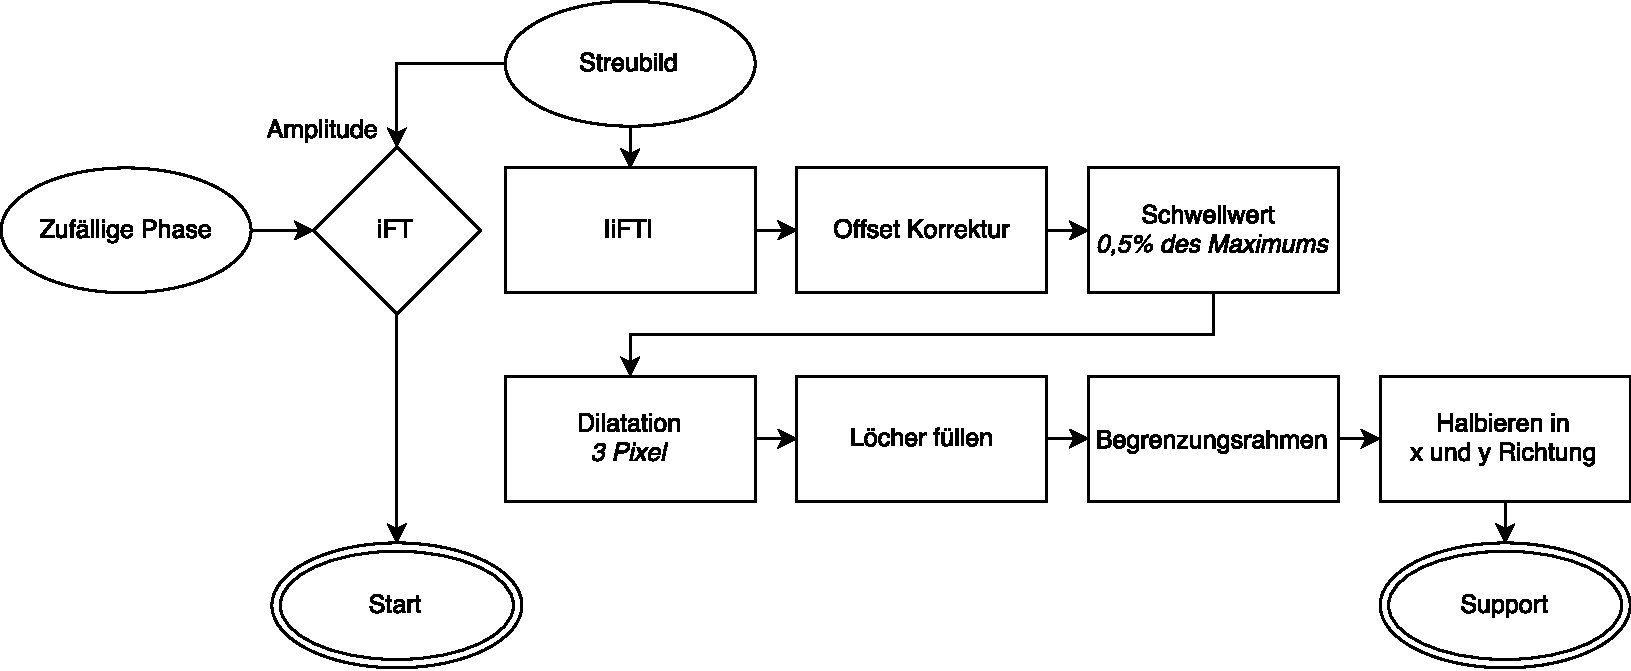
\includegraphics[width=.85\textwidth]{images/flow_genericsupport.pdf}
	\caption[Initialer Support für Shrinkwrap]{Initialer Support und Startwerte für Shrinkwrap: Ausgehend vom Betrag der inversen Fouriertransformation des Streubilds wird nach einer Offset-Korrektur mit einem Schwellwert vom 0,5\% der maximalen Intensität maskiert. Nach Dilatation um \SI{3}{Pixel} und einem Auffüllen von Löchern wird der Begrenzungsrahmen der Autokorrelation bestimmt. Der Support ist der in beiden Richtungen halbierte Begrenzungsrahmen. Die Startwerte sind die inverse Fouriertransformation der Kombination aus dem Streubild sowie zufälligen Phasen.}
	\label{fig:flow_genericsupport}
\end{figure} 

\begin{figure}
	\centering
	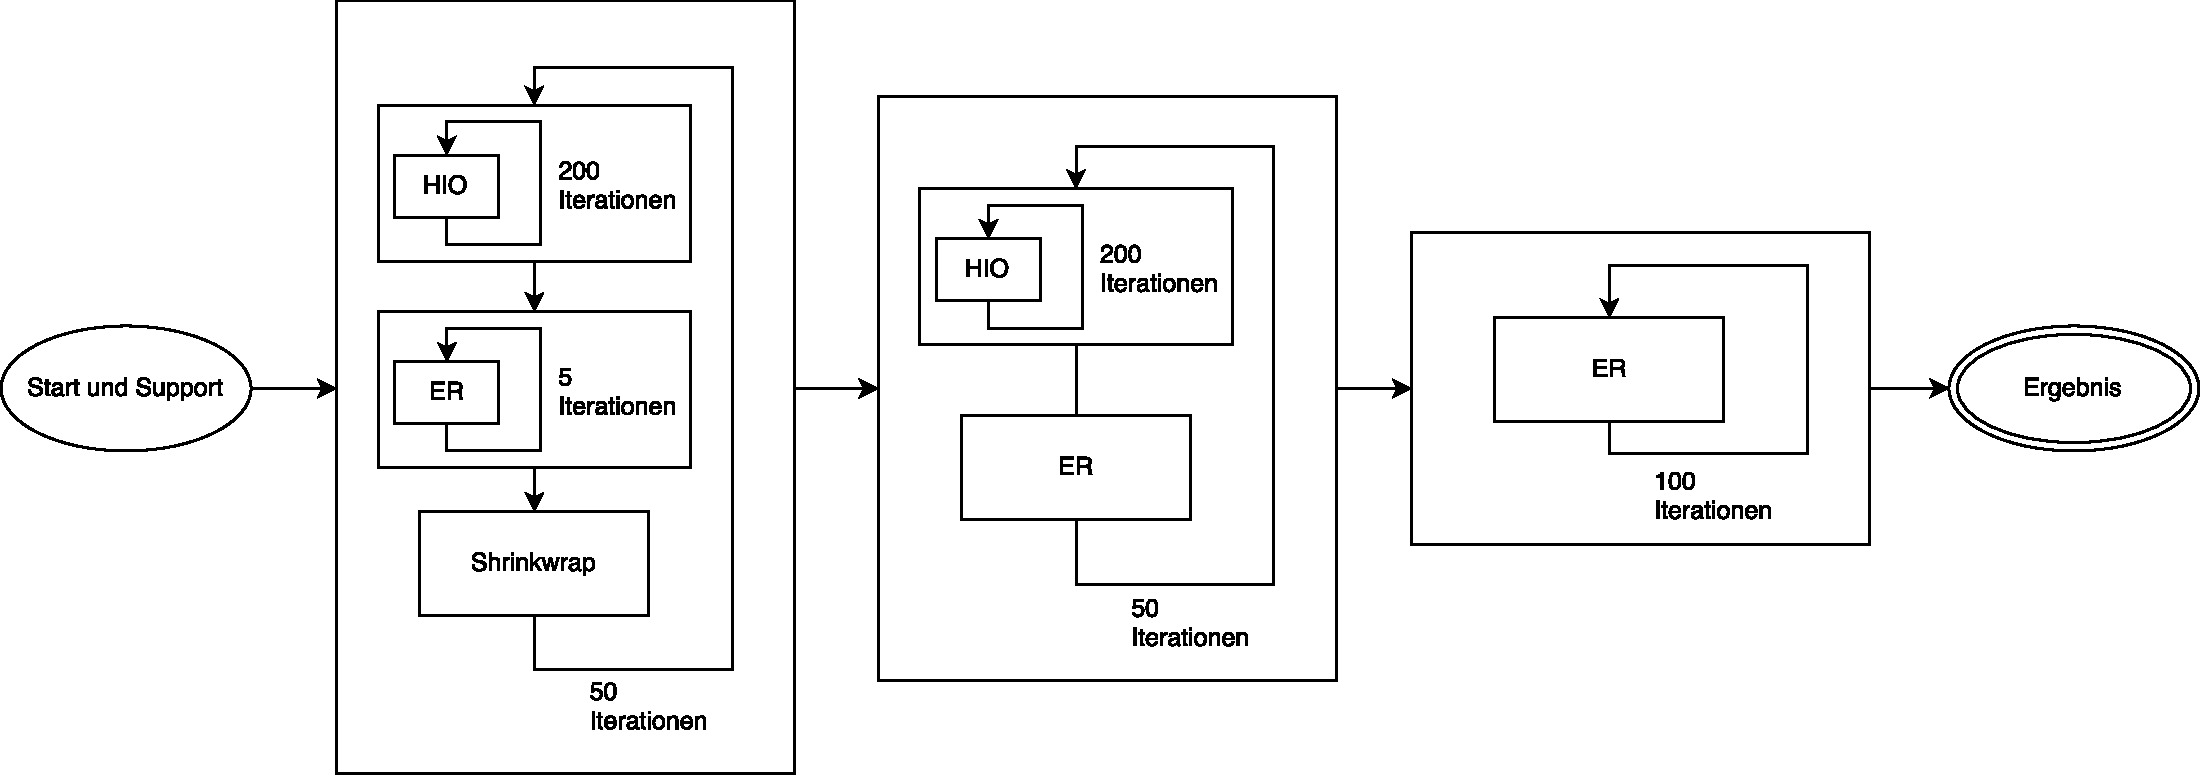
\includegraphics[width=1\textwidth]{images/flow_sw.pdf}
	\caption[Ablauf IPR mit Shrinkwrap]{Ablauf IPR mit Shrinkwrap: Ausgehend vom initialen Support sowie dem Startbild wird zunächst eine Shrinkwrap Phase durchgeführt. Diese besteht aus 50 Iterationen von jeweils 200 Iterationen HIO, 5 Iterationen ER und einem Shrinkwrap Schritt (mit den Parametern \textit{$\sigma$} und \textit{threshold}). Anschließend folgt die Rekonstruktion mit 50 Iterationen von jeweils 200 Iterationen HIO und einer Iteration ER. Die letzte Phase besteht aus einer Optimierung durch 100 Iterationen ER.}
	\label{fig:flow_sw}
\end{figure} 

\begin{figure}
	\centering
	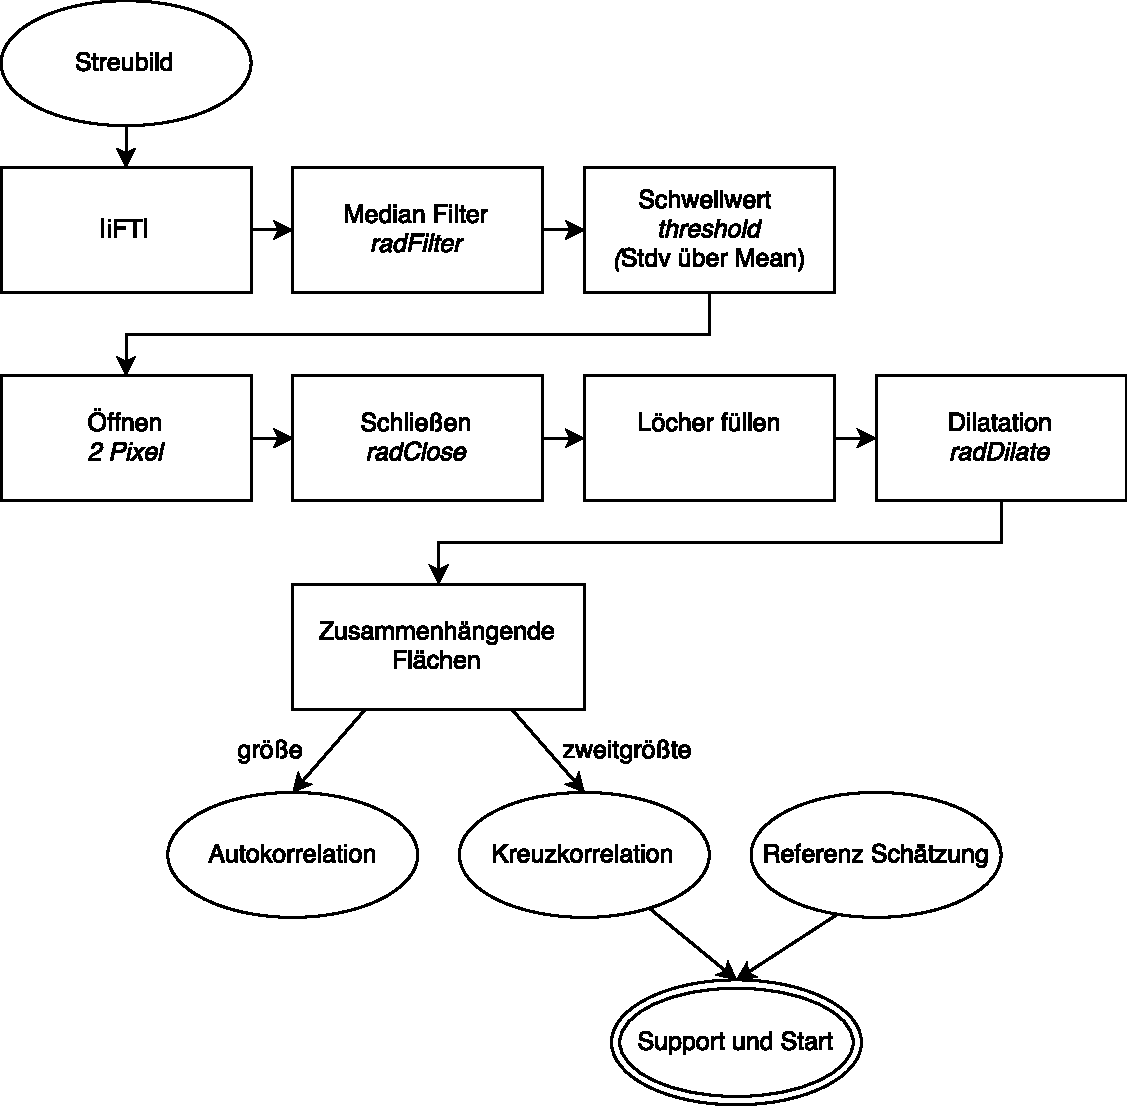
\includegraphics[width=.65\textwidth]{images/flow_holosupport.pdf}
	\caption[Support mittels Holographie]{Erzeugung des Supports und der Startwerte mittels Holographie: Ausgehend vom Betrag der inversen Fouriertransformation des Streubilds wird zunächst ein Medianfilter (mit dem Radius \textit{radFilter}) zur Rauschunterdrückung angewendet. Das Ergebnis wird mittels eines Schwellwertes, angegeben als Vielfache (\textit{threshold}) der Standardabweichung über dem Mittelwert, maskiert. Durch morphologisches Öffnen mit einem Radius von \SI{2}{Pixeln} werden einzelne Pixel eliminiert. Das Ergebnis wird morphologisch geschlossen (mit dem Radius \textit{radClose}) und die Löcher in der Maske ausgefüllt. Anschließend findet zur Supportvergrößerung eine Dilatation (mit dem Radius \textit{radDilate}) statt. Die größte zusammenhängende Fläche in dem Ergebnis ist die Maske der Autokorrelation, die zweitgrößte die Maske einer der Kreuzkorrelationen. Die Maske der Kreuzkorrelation wird mit der Referenzabschätzung zum Support, die der Kreuzkorrelation zugrunde liegenden Werte zu den Startwerten kombiniert. Die Kreuzkorrelation wird darüber hinaus für die Entfaltung genutzt.}
	\label{fig:flow_holosupport}
\end{figure} 

\begin{table}[]
	\centering
	\caption{Parameter für die iterativen Rekonstruktionsansätze}
	\label{tab:param}
	\begin{tabular}{llll}
		\hline
		\multicolumn{2}{l}{Parameter} &2D Rekonstruktionen&3D Rekonstruktionen\\ 
		\hline
		\multirow{4}{*}{Support Holographie}&\textit{radFilter} & \SI{15}{Pixel} & \SI{15}{Pixel}\\
											&\textit{threshold} & 0,66           & 1,00\\
											&\textit{radClose}  & \SI{30}{Pixel} & \SI{30}{Pixel}\\
											&\textit{radDilate} & \SI{10}{Pixel} & \SI{10}{Pixel}\\
		\hline
		\multirow{2}{*}{Support Shrinkwrap}			&Schwellenwert      & 5\,\% des Max. & 5\,\% des Max.\\
											&Filterradius       & \SI{4}{Pixel}  & \SI{10}{Pixel}\\                
		\hline
	\end{tabular}
\vspace{1cm}
\end{table}




\begin{figure}
	\centering
	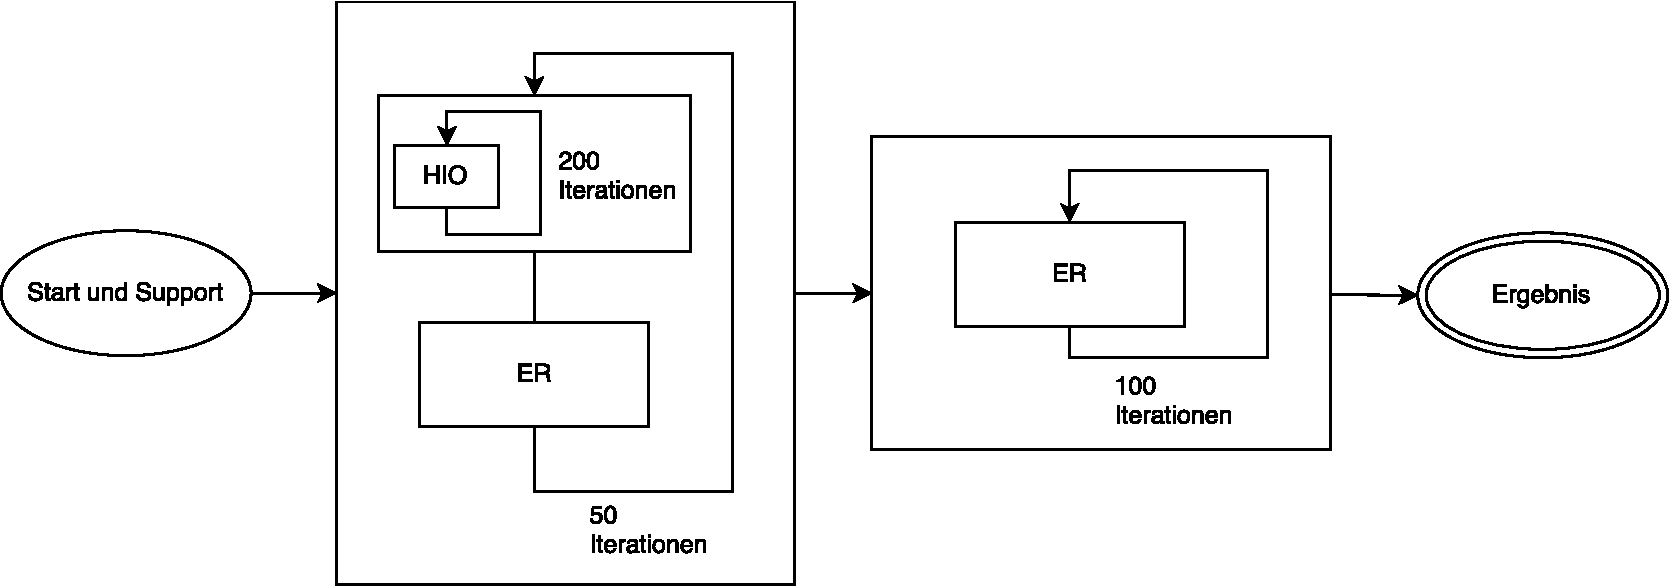
\includegraphics[width=.8\textwidth]{images/flow_holo.pdf}
	\caption[Ablauf IPR mit Holographie]{Ablauf IPR mit Shrinkwrap: Ausgehend vom mittels Holographie erstellten Support sowie dem Startbild erfolgt die Rekonstruktion mit 50 Iterationen von jeweils 200 Iterationen HIO und einer Iteration ER, gefolgt von einer Optimierung durch 100 Iterationen ER.}
	\label{fig:flow_holo}
\end{figure} 

\FloatBarrier

Die Rekonstruktionen der komplexen Austrittswellen laufen ähnlich zu den zweidimensionalen ab, es werden jedoch geringfügig andere, ebenfalls in \fref{tab:param} dargestellten Parameter genutzt. Auch hier wird für die Entfaltung der Radius der Dilatation bei der Identifikation der Kreuzkorrelation auf \SI{50}{Pixel} erhöht. Der Parameter $N$ der wird bei der Entfaltung der Austrittswelle so gewählt, dass das Ergebnis optisch optimal ist. Das Ergebnis bei zu großem sowie zu kleinem $N$ ist zum Vergleich in \fref{fig:recon3dwienernoise} dargestellt.

\begin{figure}
	\centering
	\triimage{[width=.75\textwidth]{images/recon3d-v2_wienernoise.png}}
	\caption[Wahl des Parameters bei Wiener-Entfaltung]{Zur Wahl des Parameters bei Wiener-Entfaltung: Wird der Parameter $N$ der Wiener-Entfaltung mit \num{1e2} zu klein gewählt (a), so überwiegen Störungen. Wird er mit \num{1e6} zu groß gewählt, so entsteht ein unscharfes Ergebnis (c) im Vergleich zur Verwendung des optimalen Wertes (b) von \num{1e4}.}
	\label{fig:recon3dwienernoise}
\end{figure}
